\documentclass[english,9pt]{beamer}

\usepackage{amsmath} % load this before unicode-math
\usepackage{amssymb}
%\usepackage{unicode-math}

\usepackage{fontspec}
\setmonofont{DejaVu Sans Mono}
%\setmathfont{STIXMath}
%\setmathfont{TeX Gyre Termes Math}

\usefonttheme[onlymath]{serif}

\setlength{\parskip}{\smallskipamount}
\setlength{\parindent}{0pt}

\setbeamersize{text margin left=5pt, text margin right=5pt}

\usepackage{amsmath}
\usepackage{amssymb}
\usepackage{braket}

\usepackage{minted}
\newminted{julia}{breaklines,fontsize=\scriptsize,texcomments=true}
\newminted{python}{breaklines,fontsize=\scriptsize,texcomments=true}
\newminted{bash}{breaklines,fontsize=\scriptsize,texcomments=true}
\newminted{text}{breaklines,fontsize=\scriptsize,texcomments=true}

\newcommand{\txtinline}[1]{\mintinline[fontsize=\scriptsize]{text}{#1}}
\newcommand{\jlinline}[1]{\mintinline[fontsize=\scriptsize]{julia}{#1}}

\definecolor{mintedbg}{rgb}{0.95,0.95,0.95}
\usepackage{mdframed}

\BeforeBeginEnvironment{minted}{\begin{mdframed}[backgroundcolor=mintedbg]}
\AfterEndEnvironment{minted}{\end{mdframed}}

\setcounter{secnumdepth}{3}
\setcounter{tocdepth}{3}

\makeatletter

 \newcommand\makebeamertitle{\frame{\maketitle}}%
 % (ERT) argument for the TOC
 \AtBeginDocument{%
   \let\origtableofcontents=\tableofcontents
   \def\tableofcontents{\@ifnextchar[{\origtableofcontents}{\gobbletableofcontents}}
   \def\gobbletableofcontents#1{\origtableofcontents}
 }

\makeatother

\usepackage{babel}

\begin{document}


\title{\texttt{PWDFT.jl}: Density Functional Theory Calculations with Julia}
\author{Fadjar Fathurrahman}
\institute{
Engineering Physics Department \\
Research Center for Nanoscience and Nanotechnology \\
Institut Teknologi Bandung
}
%\date{20 April 2018}
\date{24 September 2019}

\frame{\titlepage}

\begin{frame}
\frametitle{Software packages for DFT calculations}

There are a lot of software packages for DFT calculations, for examples:
\begin{itemize}
\item Quantum ESPRESSO
\item VASP
\item ABINIT
\item Gaussian series: G03, G09, G16
\item NWchem
\end{itemize}

Test math:
\begin{equation}
\alpha + \beta \oint
\end{equation}


More extensive list:
{\scriptsize
\url{https://en.wikipedia.org/wiki/List_of_quantum_chemistry_and_solid-state_physics_software}
}

\end{frame}


\begin{frame}
\frametitle{Problems}

\begin{itemize}
\item These packages are very helpful for doing various calculations based on DFT.
%
These packages are suitable for black-box-type calculations where we are only concerned about the results.
%
\item However they are generally rather difficult to extend.
  \begin{itemize}
  \item New development on the DFT functionals:
  users generally need to wait for the next release of the package to use them
  (if these functionals are to be implemented at all).
  \item Custom calculations or post-processing steps:
  Users need to know in some detail
  about how the data they are interested in is represented or implemented in the package's source code.
  \end{itemize}
\end{itemize}

\end{frame}


\begin{frame}
\frametitle{Write another DFT package?}

Personal motivation:

learning how DFT or Kohn-Sham equations are solved

frustation when trying to extend available package

\end{frame}



\begin{frame}
\frametitle{Programming languages for DFT}
    
Programming languages used:
\begin{itemize}
\item Fortran and/or C/C++: ABINIT, VASP, Quantum Espresso, ...
\item Python: GPAW
\item MATLAB: KSSOLV, RESCU
\end{itemize}
    
Static languages: Fortran, C/C++

Dynamic languages: Python and MATLAB

\end{frame}



\begin{frame}
\frametitle{Julia programming language}

A rather new programming language (2012)

Syntax is familar to MATLAB or Python users

support for multidimensional array and linear algebra

Loop is fast!

\end{frame}



\begin{frame}
\frametitle{Introducing PWDFT.jl}

\begin{itemize}
\item A program package for doing DFT calculations using Julia
\item plane wave basis + pseudopotentials (norm-conserving)
\item LDA and GGA functionals can be used (via LibXC)
\item symmetry detection (via SPGLIB)
\item algorithms for solving KS problem: SCF and Emin (PCG and DCM)
\end{itemize}

\end{frame}


\begin{frame}
\frametitle{Aims}

\begin{itemize}
\item Friendly-to-developers DFT package: enables quick implementation of various algorithms
\item educational purpose: simple yet powerful enough to carry out practical DFT calculations
for molecular and crystalline systems.
\end{itemize}

\end{frame}

\begin{frame}[plain]
\begin{center}
\Huge{Examples}
\end{center}
\end{frame}

\begin{frame}
\frametitle{Typical steps}

Write Julia code not an input file.

Typical steps:
\begin{itemize}
\item Initialize Atoms
\item Initialize Hamiltonian with the given Atoms
\item Solve the Hamiltonian
\end{itemize}

Atomic units are used (energy: Hartree, length: bohr)

\end{frame}


\begin{frame}[fragile]
\frametitle{Example: hydrogen molecule in a box}

{\centering
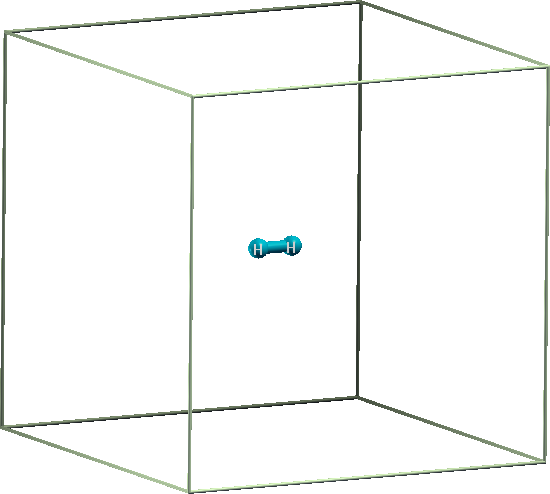
\includegraphics[width=0.25\textwidth]{codes/H2/H2.png}

}

\begin{juliacode}
using PWDFT # activate PWDFT package

# Initialize an H2 molecule in cubic box (simple cubic lattice)
# The coordinates are read from
atoms = Atoms( xyz_file="H2.xyz",
               LatVecs=gen_lattice_sc(16.0) )

pspfiles = ["H-q1.gth"] # pseudopotential parameters

ecutwfc = 15.0 # cutoff energy for wave function expansion

# initialize Hamiltonian
Ham = Hamiltonian( atoms, pspfiles, ecutwfc )

# solve the Kohn-Sham problem (using SCF algorithm)
KS_solve_SCF!( Ham )
\end{juliacode}


\end{frame}


\begin{frame}[fragile]
\frametitle{Output}

\begin{textcode}
$ julia run.jl 

Self-consistent iteration begins ...
update_psi = LOBPCG
mix_method = simple
Density mixing with betamix =    0.20000
    
-------------------------------------------------------
       iter            E            ΔE           Δρ
-------------------------------------------------------
SCF:     1      -0.9088890376  9.08889e-01  1.36287e-04
SCF:     2      -0.9197780666  1.08890e-02  1.17877e-04
SCF:     3      -0.9589404606  3.91624e-02  9.53668e-05
SCF:     4      -0.9975511159  3.86107e-02  7.60953e-05
.... # snipped
\end{textcode}

\end{frame}


\begin{frame}[fragile]
\frametitle{Converged Kohn-Sham energy components}

\begin{columns}[T]

\begin{column}{0.45\textwidth}
PWDFT.jl's result:
\begin{textcode}
-------------------------
Final Kohn-Sham energies:
-------------------------

Kinetic    energy:       1.0100082069
Ps_loc     energy:      -2.7127851088
Ps_nloc    energy:       0.0000000000
Hartree    energy:       0.9015229089
XC         energy:      -0.6314259148
PspCore    energy:      -0.0000012675
-------------------------------------
Electronic energy:      -1.4326811753
NN         energy:       0.3131700043
-------------------------------------
Total      energy:      -1.1195111709
\end{textcode}
\end{column}

\begin{column}{0.55\textwidth}

ABINIT's result:
\begin{textcode}
Components of total free energy (in Hartree) :

   Kinetic energy  =  1.01004059294567E+00
   Hartree energy  =  9.01545039301481E-01
   XC energy       = -6.31436384237843E-01
   Ewald energy    =  3.13170052325859E-01
   PspCore energy  = -1.26742500464741E-06
   Loc. psp. energy= -2.71283243086241E+00
   NL   psp  energy=  0.00000000000000E+00
   >>>>>>>>> Etotal= -1.11951439795224E+00
\end{textcode}
\end{column}

\end{columns}

\end{frame}

\begin{frame}
\frametitle{SCF solvers}

Kohn-Sham problem is solved using self-consistent field (SCF) iterations.
This is the most popular method.

In PWDFT.jl we can set various options to SCF algorithm:

\begin{itemize}
\item \jlinline{betamix}: linear mixing parameters (between 0 and 1)
\item \jlinline{mix_method}: linear, adaptive linear, Anderson, Pulay, restarted Pulay, periodic Pulay,
  and Broyden.
\item \jlinline{update_psi}: how to update the wave functions (iterative diagonalization or Chebyshev
subspace filtering).
\end{itemize}


\end{frame}

\begin{frame}
\frametitle{Direct energy minimization}

For systems with band gaps:

Conjugate gradient

Direct minimization

\end{frame}

\end{document}

